\documentclass{beamer}

\usepackage[utf8]{inputenc}
%\usepackage{beamerthemesplit}
\usepackage{url}
\usepackage{tikz}
\usepackage{alltt}
\usepackage{listings}
\usepackage{marvosym}
\usepackage{color}
\usepackage[multidot]{grffile}
\usepackage{multirow}
\usepackage{array}
\usepackage{setspace}
\usepackage{hyperref}
\usepackage{verbatim}
\usepackage{fancyvrb}
%\hypersetup{colorlinks=true, linkcolor=blue,  anchorcolor=blue,  
%citecolor=blue, filecolor=blue, menucolor=blue, pagecolor=blue,  
%urlcolor=blue} 
\lstset{keywordstyle=\bfseries\color{brown},
        stringstyle=\ttfamily,
        commentstyle=\color{blue}\textit,
        showstringspaces=false}

\useoutertheme{}
\usetheme{Madrid}
\graphicspath{{pics/}{global/}
{pics/I/}{pics/A1/}{pics/A2/}{pics/A3/}{pics/A4/}{pics/A5/}{pics/A6/}{pics/A7/}
}

\logo{
\includegraphics[height=1cm]{ProcessHorizontal}} 

\institute{Center for Computation and Technology\\Louisiana State University, Baton Rouge, LA}

\setbeamertemplate{navigation symbols}{} 

\title{CSC 7700: Scientific Computing}

% We want to use the infolines outer theme because it does not use a lot of
% space, but it also tries to print an institution and the slide
% numbers (which we might not want to show). Therefore, we here redefine the
% footline ourselfes - mostly a copy & paste from
% /usr/share/texmf/tex/latex/beamer/themes/outer/beamerouterthemeinfolines.sty
\defbeamertemplate*{footline}{infolines theme without institution and slide numbers}
{
  \leavevmode%
  \hbox{%
  \begin{beamercolorbox}[wd=.25\paperwidth,ht=2.25ex,dp=1ex,center]{author in head/foot}%
    \usebeamerfont{author in head/foot}\insertshortauthor
  \end{beamercolorbox}%
  \begin{beamercolorbox}[wd=.5\paperwidth,ht=2.25ex,dp=1ex,center]{title in head/foot}%
    \usebeamerfont{title in head/foot}\insertshorttitle
  \end{beamercolorbox}%
  \begin{beamercolorbox}[wd=.25\paperwidth,ht=2.25ex,dp=1ex,center]{date in head/foot}%
    \usebeamerfont{date in head/foot}\insertshortdate{}
  \end{beamercolorbox}}%
  \vskip0pt%
}

% Some useful commands
\newcommand{\abspic}[4]
 {\vspace{ #2\paperheight}\hspace{ #3\paperwidth}\includegraphics[height=#4\paperheight]{#1}\\
  \vspace{-#2\paperheight}\vspace{-#4\paperheight}\vspace{-0.0038\paperheight}}

\newcommand{\picw}[4]{{
 \usebackgroundtemplate{
 \color{black}\vrule width\paperwidth height\paperheight\hspace{-\paperwidth}\hspace{-0.01\paperwidth}
 \hspace{#4\paperwidth}\includegraphics[width=#3\paperwidth, height=\paperheight]{#1}}\logo{}
 \frame[plain]{\frametitle{#2}}
}}
\newcommand{\pic}[2]{\picw{#1}{#2}{}{0}}

\newcommand{\question}[1]{\frame{\frametitle{#1}
 \begin{centering}\Huge #1\\\end{centering}
}}



\subtitle[Module A]{{\large Module A: Basic Skills}\\*[0.3em]Lecture 3: Record and share your work: revision control systems}
\author[\mbox{
\includegraphics[height=0.6em]{fl_300}\hspace{0.5em}Frank Löffler}]{Dr Frank Löffler}
\date{Sep 06 2013}
\usecolortheme[RGB={124,0,188}]{structure}

\begin{document}

\frame{\titlepage}

\section{Overview}
\frame{\frametitle{}\begin{centering}\LARGE\insertsectionhead\\\end{centering}}


\frame[containsverbatim]{ \frametitle{Version control systems}
 Version Control Systems:
 \begin{itemize}
  \item Most commonly stand-alone applications
  \item Also embedded into various other software, e.g.
   \begin{itemize}
    \item word processors
    \item spreadsheets
    \item content management systems
    \item wikis
   \end{itemize}
 \end{itemize}
 Changes:
 \begin{itemize}
  \item Might be identified by number or letter code
  \item Termed as ``revision number'', ``revision level'', or simply ``revision''
  \item Associated with time-stamp, user and log message
  \item Can be compared, restored, and with some types of files, merged
 \end{itemize}
}

\frame[containsverbatim]{ \frametitle{Version control systems}
 Traditionally: centralized model - solve conflicts with one of two methods:
 \begin{itemize}
  \item File locking
   \begin{itemize}
    \item grant write access to only one checkout at a time
    \item benefit: can provide some protection against difficult conflicts
    \item drawback: when locked for too long, developers are tempted to bypass system
   \end{itemize}
  \item Version merging
   \begin{itemize}
    \item Simultaneous edit by multiple developers allowed
    \item Merge necessary when transferring change to central server
    \item Automatic merging available for simple files: text
   \end{itemize}
 \end{itemize}
 Often both options are available, but locking is typically not used (anymore).
}

\frame[containsverbatim]{ \frametitle{Branches - Trunk - Tags}
 \begin{minipage}{0.6\linewidth}
 Branch
 \begin{itemize}
  \item Duplication of a (larger) object under revision control
  \item Usually complete directory tree
 \end{itemize}
 Trunk / Master
 \begin{itemize}
  \item Main, central development branch
  \item Upstream branch
 \end{itemize}
 Tag
 \begin{itemize}
  \item Repository snapshots
  \item Used especially for releases
  \item Synonyms: labels, baselines
 \end{itemize}
 Some repository systems treat all three\\identically.
 \end{minipage}
 \begin{minipage}{0.35\linewidth}
  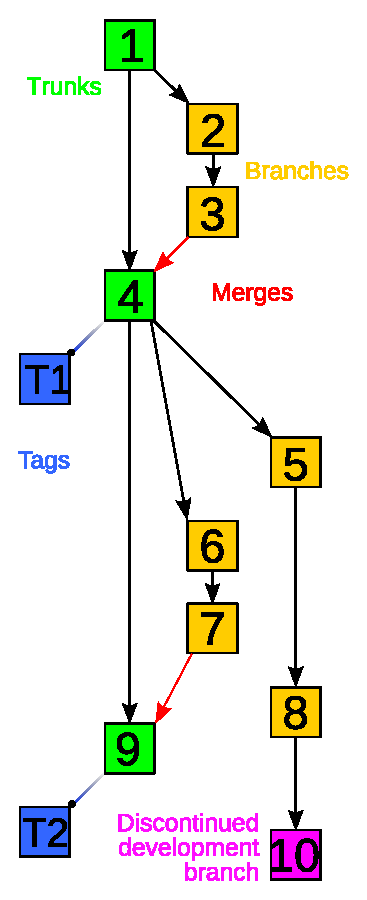
\includegraphics[height=7cm]{Revision_controlled_project_visualization-2010-24-02}\\
 \end{minipage}\\
}

\frame[containsverbatim]{ \frametitle{Version control systems - Branches}
 Branching: duplication of an object under revision control
 \begin{itemize}
  \item Modifications can happen in parallel along multiple branches.
  \item Branch: also known as trees, streams or code-lines
  \item Originating branch: \textit{parent} branch or \textit{upstream}
  \item Branch without parent: \textit{trunk} or \textit{mainline}
  \item Branches might be merged, especially into \textit{trunk}
  \item Branches not intended to be merged usually called \textit{fork}
 \end{itemize}
}

\frame[containsverbatim]{ \frametitle{Distributed revision control}
 \begin{itemize}
  \item Peer-to-peer approach
  \item Theoretically no central repository
  \item Repositories synchronized by exchanging change-sets (patches)
  \item Communication only necessary for exchange with other copies
  \item Some common operations are fast, because local
  \item In practice, projects tend to have one designated central,
        ``official'' repository and only limited exchange between user copies.
 \end{itemize}
}

\frame[containsverbatim]{ \frametitle{Checkouts - Exports - Update - Commits}
 Checkout (synonym: working copy)
 \begin{itemize}
  \item Act of creating a local working copy from the repository
  \item User may specify a specific revision or obtain the latest
 \end{itemize}
 Export
 \begin{itemize}
  \item Act of obtaining only files from the repository
  \item Similar to checkout, but creates clean directory tree without version control metadata.
 \end{itemize}
 Update
 \begin{itemize}
  \item Merges changes in the repository into the local working copy
  \item Might create conflicts with local changes that might have to be resolved manually
 \end{itemize}
 Commit
 \begin{itemize}
  \item Action of writing or merging the changes made in the working copy back to the repository.
  \item Might not be possible without an up-to-date checkout
  \item Also: New revision that is created by committing
 \end{itemize}
}

\frame[containsverbatim]{ \frametitle{Some day on Geek \& Poke}
 \begin{centering}
  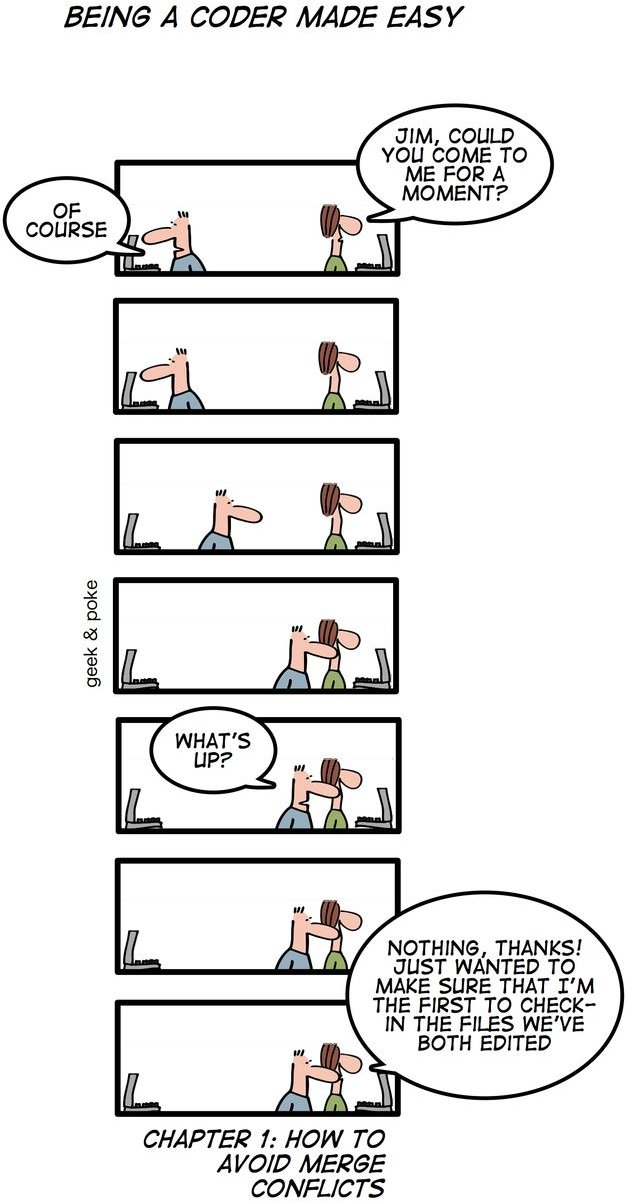
\includegraphics[height=8cm]{geek_and_poke_merge_conflicts}\\
 \end{centering}
 \tiny http://geekandpoke.typepad.com/
}

\frame[containsverbatim]{ \frametitle{Revision control - Log messages}
 ``\textit{If you have nothing to say about what you are committing, you have nothing to commit.}''\\*[0.5em]
 Log messages serve at least three important purposes
 \begin{itemize}
  \item To speed up the reviewing process.
  \item To help to write a good release note.
  \item To help the future maintainers to find out why a particular change was made
        (that might be you!)
 \end{itemize}
 At least try to
 \begin{itemize}
  \item Summarize clearly in one line what this commit is about
  \item Describe the change, not how it was made
 \end{itemize}
 Even better
 \begin{itemize}
  \item Write one-line summary, followed by an empty line and a longer description
  \item Line-break the commit message
 \end{itemize}
}

\frame[containsverbatim]{ \frametitle{Some day on Geek \& Poke}
 \begin{centering}
  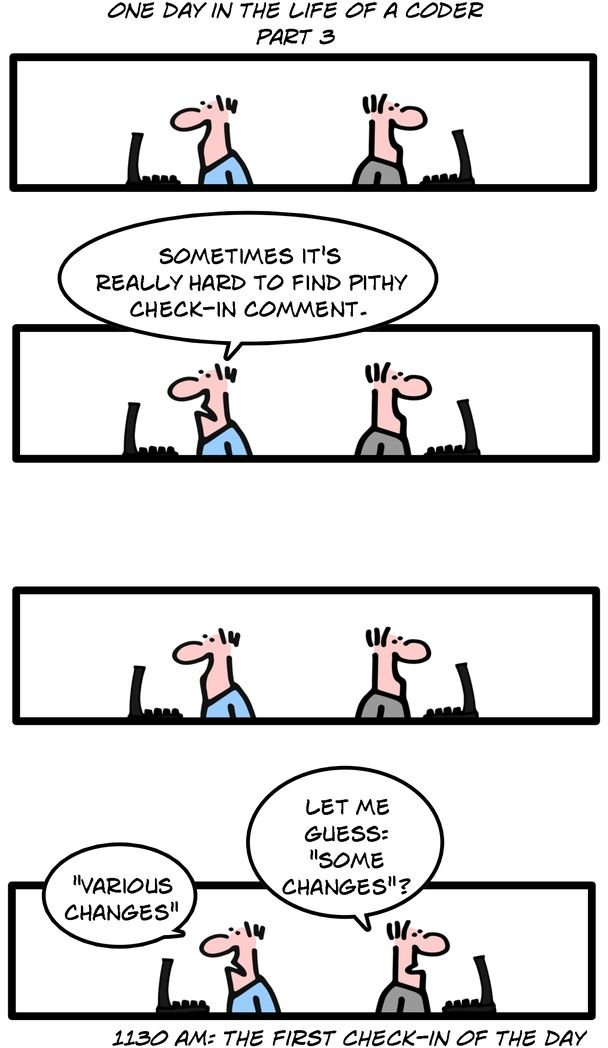
\includegraphics[height=8cm]{geek_and_poke_commit_messages}\\
 \end{centering}
 \tiny http://geekandpoke.typepad.com/
}

\frame[containsverbatim]{ \frametitle{Revision control - example work-flows}
 Simple change to central repository
 \begin{enumerate}
  \item Checkout
  \item Change file locally
  \item Test change
  \item Update - shows no remote changes
  \item Commit change
 \end{enumerate}
}

\frame[containsverbatim]{ \frametitle{Revision control - example work-flows}
 Change to central repository with conflicts
 \begin{enumerate}
  \item Checkout
  \item Change file locally
  \item Test change
  \item Update shows changes and merge conflicts
  \item Resolve conflict
  \item Test change
  \item Repeat updating until success
  \item Commit change
 \end{enumerate}
}

\frame[containsverbatim]{ \frametitle{Revision control - Conflicts}
 Updating from repository will
 \begin{itemize}
  \item Try to merge remote changes with local changes
  \item Create a conflict if this fails
   \begin{itemize}
    \item Binary files: only option between 'theirs full' and 'mine full'
    \item Text files: fine-grained control of multiple changes in single file
   \end{itemize}
 \end{itemize}
 Example:\\*[1em]
 \begin{minipage}{0.5\linewidth}
  \begin{verbatim}
$svn update
  U index.html
  G changed-b.html
  C rubbish-b.html
  Updated to revision 46.
  \end{verbatim}
 \end{minipage}
 \begin{minipage}{0.45\linewidth}
  \begin{itemize}
   \item U - Updated
   \item G - Merged
   \item C - Conflict
  \end{itemize}
 \end{minipage}
 \begin{itemize}
  \item Test after conflict resolving!
 \end{itemize}
}

\frame[containsverbatim]{ \frametitle{Some day on Geek \& Poke}
 \begin{centering}
  
\includegraphics[height=8cm]{geek_and_poke_svn_update}\\
 \end{centering}
 \vspace{-0.5cm}\tiny http://geekandpoke.typepad.com/
}

\frame[containsverbatim]{ \frametitle{Some day on Geek \& Poke}
 \begin{centering}
  
\includegraphics[height=8cm]{geek_and_poke_svn_update2}\\
 \end{centering}
 \vspace{-0.5cm}\tiny http://geekandpoke.typepad.com/
}

\frame[containsverbatim]{ \frametitle{Revision control - Conflicts}
 Conflict markers in text files:
\begin{verbatim}
<<<<<<< filename
    your changes
=======
    code merged from repository
>>>>>>> revision
\end{verbatim}
 Resolve conflict by
 \begin{itemize}
  \item Reviewing both changes and manually merging them
  \item Test merged version
  \item Tell RCS that conflict is resolved
  \item Commit
 \end{itemize}
}

\frame[containsverbatim]{ \frametitle{Some day on Geek \& Poke}
 \begin{centering}
  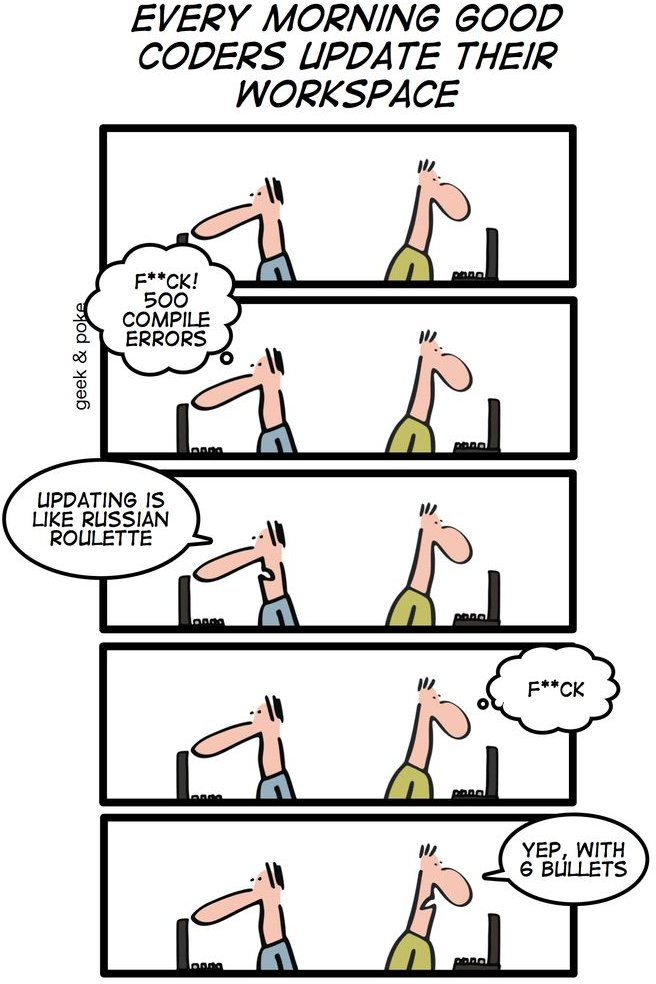
\includegraphics[height=8cm]{geek_and_poke_russion_roulette}\\
 \end{centering}
 \vspace{-0.5cm}\tiny http://geekandpoke.typepad.com/
}

\frame[containsverbatim]{ \frametitle{Some day on Geek \& Poke}
 \begin{centering}
  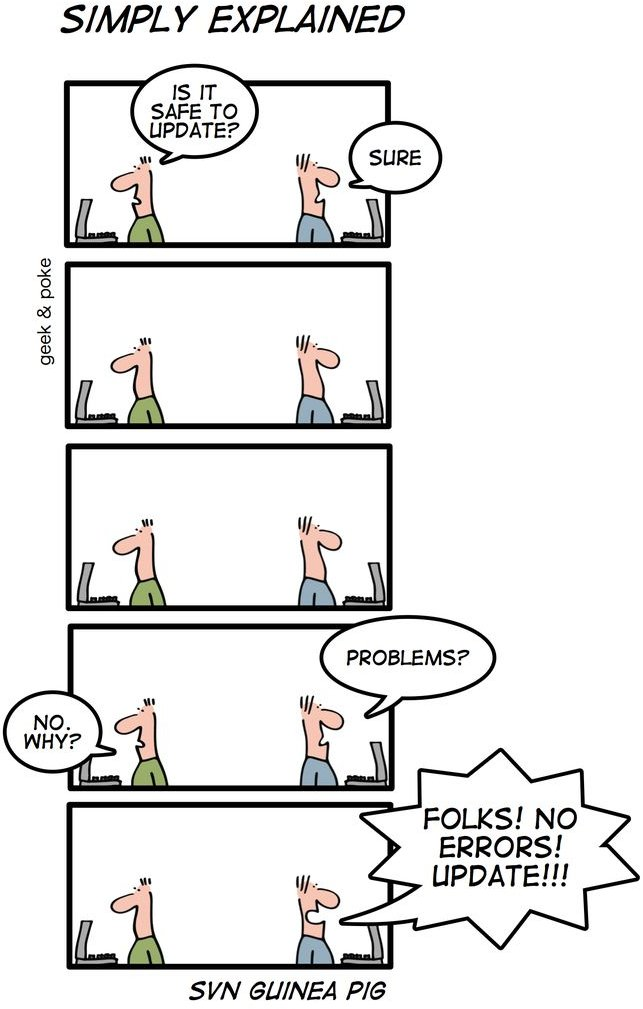
\includegraphics[height=8cm]{geek_and_poke_svn_guinea_pig}\\
 \end{centering}
 \vspace{-0.5cm}\tiny http://geekandpoke.typepad.com/
}

\frame[containsverbatim]{ \frametitle{Revision control - example workflows}
 Simple branch example
 \begin{enumerate}
  \item Create branch from trunk
  \item Checkout branch
  \item Change files locally, test and commit like on trunk
  \item Possibly merge changes from trunk, resolve conflicts as usual
  \item Eventually, merge changes from branch back into trunk
  \item Remove branch
 \end{enumerate}
}

\frame[containsverbatim]{ \frametitle{Revision control - example workflows}
 Applying change using distributed RCSs
 \begin{enumerate}
  \item Checkout / Clone
  \item Change file locally
  \item Test change
  \item Commit change (locally)
  \item Update from other working copy (e.g. ``central'' repository)
  \item Resolve possible conflicts, commit needed changes
  \item Test again
  \item Repeat until success
  \item Push commit(s) to other working copy (e.g. ``central`` repository)
 \end{enumerate}
}

\frame[containsverbatim]{ \frametitle{Revision control - history examination}
 History in RCSs can be used to find out
 \begin{itemize}
  \item Why something was implemented (log messages)
  \item When something was implemented
  \item Who did a certain change
 \end{itemize}
 Typical example:
 \begin{itemize}
  \item Test of checkout: ok
  \item Test of checkout after local changes: ok
  \item Test after update from repository: failure
 \end{itemize}
 Narrow down location of bug by
 \begin{itemize}
  \item List log messages since last known working version
  \item Test without some of remote changes (go back in history)
 \end{itemize}
 Tools can help with this process.
}

\frame[containsverbatim]{ \frametitle{Some day on Geek \& Poke}
 \begin{centering}
  
\includegraphics[height=8cm]{geek_and_poke_svn_blame}\\
 \end{centering}
 \vspace{-0.5cm}\tiny http://geekandpoke.typepad.com/
}
\frame[containsverbatim]{ \frametitle{Summary - Best RCS usage}
 Basic
 \begin{itemize}
  \item Use it, learn (much) about it!
  \item Put as much as possible under version control
  \item Only put original source in version control, not built objects
  \item Test changes before committing
  \item Commit often and in logical chunks
  \item Update as often as possible (close open files beforehand!)
  \item Write meaningful commit messages
 \end{itemize}
 Advanced
 \begin{itemize}
  \item Branch only when necessary
  \item Don't copy when you mean to branch
  \item Branch late
  \item Propagate / Merge early and often
 \end{itemize}
 Reading: \href{http://svnbook.red-bean.com/}{Subversion}, \href{http://www.kernel.org/pub/software/scm/git/docs/user-manual.html}{Git}, \href{http://mercurial.selenic.com/wiki/Tutorial}{Mercurial}
}

\section*{Course Work}

\frame[containsverbatim]{ \frametitle{Course Work I}
 \verb|http://cactus.cct.lsu.edu/courses/sci-comp-2013/YOURNAME/|
 \begin{itemize}
  \item Your personal subversion repository for CSC7700
  \item Commit coursework files to sub-directory \verb|coursework/LECTURE|, e.g.,
        \verb|coursework/A3/|
  \item Otherwise use as you like (be nice)
  \item Data is only accessible to all lecturers and yourself
 \end{itemize}
}

\frame[containsverbatim]{ \frametitle{Course Work II}
 \verb|https://svn.cct.lsu.edu/repos/courses/sci-comp-2013-public/|
 \vspace{-1em}
 \begin{itemize}
  \item Checkout the class repository
  \item Update it from time to time to get new and updated materials
 \end{itemize}
 \vspace{0.5em}
 \verb|http://svn.cactuscode.org/flesh/trunk/src|
 \begin{itemize}
  \item What was the commit message of revision $7$? Show how you found out.
  \item Which revision removed the macro \verb|GROUP_SCALAR|? (mentioned in the commit message)
  \item Do a checkout and an export of that repository. Report about the size of both.
        Which one is larger and why? Which version of svn are you using?
  \item Commit \textbf{PDF} report until \textbf{Sep 13 2013} to \verb|coursework/A3/|
 \end{itemize}
 \vspace{2em}
}
\end{document}

